
%%%%%%%%%%%%%%%%%%%%%%% file typeinst.tex %%%%%%%%%%%%%%%%%%%%%%%%%
%
% This is the LaTeX source for the instructions to authors using
% the LaTeX document class 'llncs.cls' for contributions to
% the Lecture Notes in Computer Sciences series.
% http://www.springer.com/lncs       Springer Heidelberg 2006/05/04
%
% It may be used as a template for your own input - copy it
% to a new file with a new name and use it as the basis
% for your article.
%
% NB: the document class 'llncs' has its own and detailed documentation, see
% ftp://ftp.springer.de/data/pubftp/pub/tex/latex/llncs/latex2e/llncsdoc.pdf
%
%%%%%%%%%%%%%%%%%%%%%%%%%%%%%%%%%%%%%%%%%%%%%%%%%%%%%%%%%%%%%%%%%%%


\documentclass[runningheads]{llncs}

\usepackage{amssymb}
\setcounter{tocdepth}{3}
\usepackage{graphicx}

\usepackage{url}
\urldef{\mailsa}\path|{aysengupta, xianlin, ksanjeev, sravichandra}@cs.stonybrook.edu|
\newcommand{\keywords}[1]{\par\addvspace\baselineskip
\noindent\keywordname\enspace\ignorespaces#1}
\newcommand{\swallow}[1]{ }

\begin{document}

\mainmatter  % start of an individual contribution

% first the title is needed
\title{Status Report: Team 8\\
Predicting the Prices of Oil and Gold}

% a short form should be given in case it is too long for the running head
\titlerunning{Predicting the Prices of Oil and Gold}

% the name(s) of the author(s) follow(s) next
%
% NB: Chinese authors should write their first names(s) in front of
% their surnames. This ensures that the names appear correctly in
% the running heads and the author index.
%
\author{Ayush Sengupta \and Benjamin Lin \and Komal Sanjeev \and Sreevathsan Ravichandran}
%
\authorrunning{Ayush Sengupta \and Benjamin Lin \and Komal Sanjeev \and Sreevathsan Ravichandran}
% (feature abused for this document to repeat the title also on left hand pages)

% the affiliations are given next; don't give your e-mail address
% unless you accept that it will be published
\institute{Department of Computer Science, Stony Brook University,\\
Stony Brook, NY 11794-4400\\
\mailsa\\
\url{http://www.cs.stonybrook.edu/~skiena/591/projects}}

%
% NB: a more complex sample for affiliations and the mapping to the
% corresponding authors can be found in the file "llncs.dem"
% (search for the string "\mainmatter" where a contribution starts).
% "llncs.dem" accompanies the document class "llncs.cls".
%

\toctitle{Lecture Notes in Computer Science}
\tocauthor{Authors' Instructions}
\maketitle

\swallow{   % DO NOT BOTHER WITH THIS
\begin{abstract}
The abstract should summarize the contents of the paper and should
contain at least 70 and at most 150 words. It should be written using the
\emph{abstract} environment.
\keywords{We would like to encourage you to list your keywords within
the abstract section}
\end{abstract}
}


\section{Background Updates} 
\subsection{Project Objective Update}

Instead of predicting the prices of oil and gold on December 1st 2014, our project objective has been updated to "Predicting the prices of Oil and Gold on January 1st 2015 as of December 1's in 2014"

\subsection{Baseline Models}

In this report, we only use the following two baseline models to be compared with our autoregressive models and autoregressive models taking economic factors to illustrate our enhancement on models.\\

\noindent\textbf{Oil price same as last day price:} $P_{t}$ = $P_{t-1}$\\
\textbf{Weighted mean of the last 3 days Oil price:} \\
$P_{t}$ = $\frac{1}{\{k(k+1)\}^2}\sum\limits_{i=1}^k (k-i+1)^3P_{t-i}$\\
\\Same baseline models used for the gold price for comparison as well.

\subsection{Autoregressive Models}
For both oil and gold price predictions, we include two simple autoregressive models "price of last 1 day" and "prices of past 3 days".
\subsubsection{ARMA Models} 
Autoregressive Moving Average (ARMA) Model is a member in the autogressive model family [CHECK]. It takes two parameters: the frist one represents the auto-regression and the second one represents the moving average [CHECK]. For oil price prediction, we implemented ARMA(2,0) and ARMA(3,1); for gold price prediction, we implemented ARMA(2,0), ARMA(3,1) and ARMA(2,2).

\subsection{Autoregressive Models taking Economic Factors into consideration}
In this phase, we have also implemented multiple linear regression models with autoregressive features on both oil and gold price predictions. \\
For oil price prediction, we take S\&P500 Index (SP500), NYSE Index (NYSE), US Dollar Index (USD), and Gold Price into consideration. For gold price prediction, we take S\&P500 Index, NYSE Index, US Dollar Index, Euro/USD Exchange Rate (EURO/USD), Consumer Sentiment Index (CSI) and Oil Price into consideration.

\subsection{Spot price prediction using Futures prices}
[KOMAL: YOU MAY PUT YOUR KNOWLEDGE ON FUTURES PRICE HERE]

\section{Data Matrices}

\subsection{Daily Data} We have Oil Price, Gold Price, SP500, NYSE, USD, CSI, EURO/USD collected. \\\\

\noindent Oil Price: 5023 rows, ranged from Oct 03, 1994 to Sept 30, 2014 \\
Gold Price: 5217 rows, ranged from Oct 03, 1994 to Sept 30, 2014 \\
SP500: 5035 rows, ranged from Oct 03, 1994 to Sept 30, 2014 \\
NYSE: 5035 rows, ranged from Oct 03, 1994 to Sept 30, 2014 \\
USD: 5029 rows, ranged from Oct 03, 1994 to Sept 30, 2014 \\
CSI: 5217 rows, ranged from Oct 03, 1994 to Sept 30, 2014 \\
EURO/USD: 5109 rows, ranged from Oct 03, 1994 to Sept 30, 2014 \\

\begin{figure}
\centering
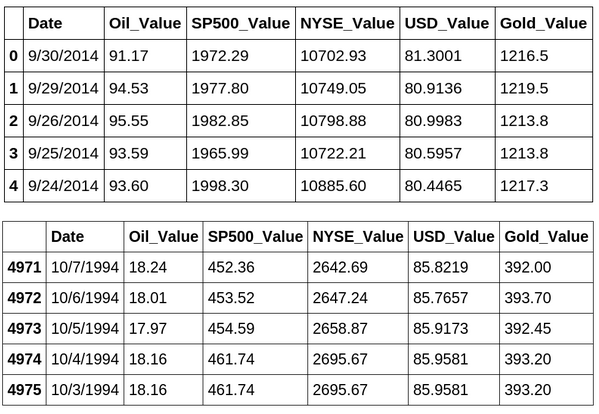
\includegraphics[width=\textwidth]{DataMatrices_Oil_Daily.png}
\caption{Data frame for oil price and its related economic factors}
\label{fig:DataMatrices_Oil_Daily.png}
\end{figure}

\begin{figure}
\centering
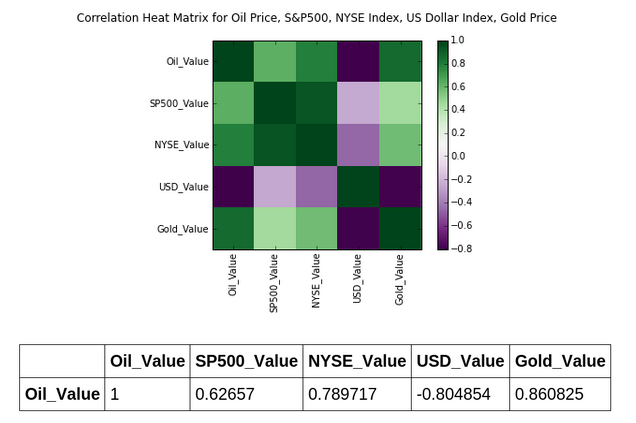
\includegraphics[width=\textwidth]{HeatMap_Oil_Daily.png}
\caption{Heat Map and Correlatin Coefficient Matrix for oil price and its related economic factors}
\label{fig:HeatMap_Oil_Daily.png}
\end{figure}

\begin{figure}
\centering
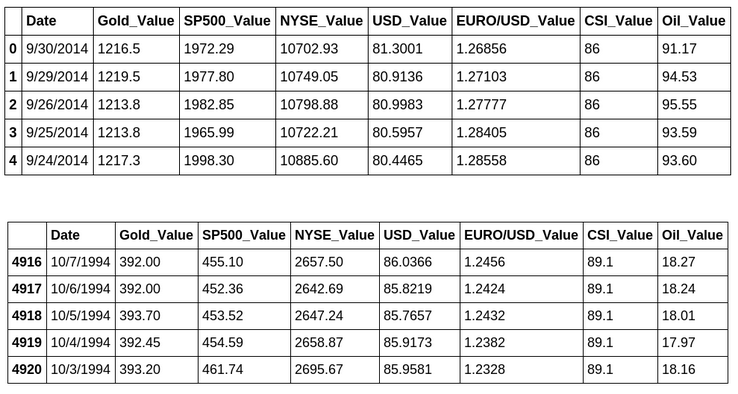
\includegraphics[width=\textwidth]{DataMatrices_Gold_Daily.png}
\caption{Data frame for gold price and its related economic factors}
\label{fig:DataMatrices_Gold_Daily.png}
\end{figure}

\begin{figure}
\centering
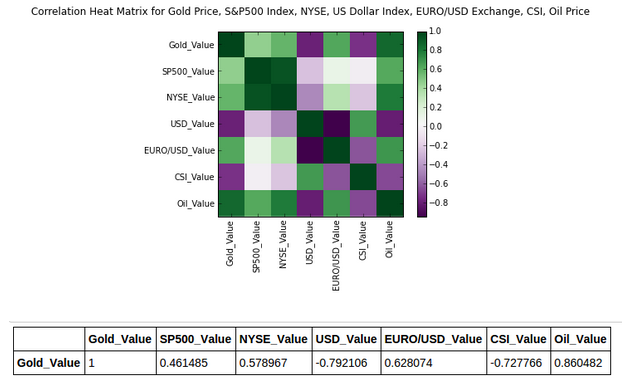
\includegraphics[width=\textwidth]{HeatMap_Gold_Daily.png}
\caption{Heat Map and Correlatin Coefficient Matrix for gold price and its related economic factors}
\label{fig:HeatMap_Gold_Daily.png}
\end{figure}

\subsection{Monthly Data} We have Oil Price, Gold Price, SP500, NYSE, USD, CSI collected. \\

\subsection{Data Source}
\noindent For both the daily and monthly data, they are obtained from \\
Oil Price: \url{https://www.quandl.com} \\ 
Gold Price: \url{https://www.quandl.com} \\
SP500: \url{https://www.quandl.com} \\
NYSE: \url{https://www.quandl.com} \\
USD: \url{https://www.quandl.com} \\
EURO/USD: \url{https://www.quandl.com} \\
CSI: \url{http://future.aae.wisc.edu/data/monthly_values/by_area/998?grid=true} \\

[ADD: HOW SATISFIED ARE YOU WITH THE DATA YOU COLLECTED?]

\section{Development/Evaluation Environment}

The model development process, taking oil price prediction using economic factors for example, can be viewed in the following flow chart: \\

\begin{figure}
\centering
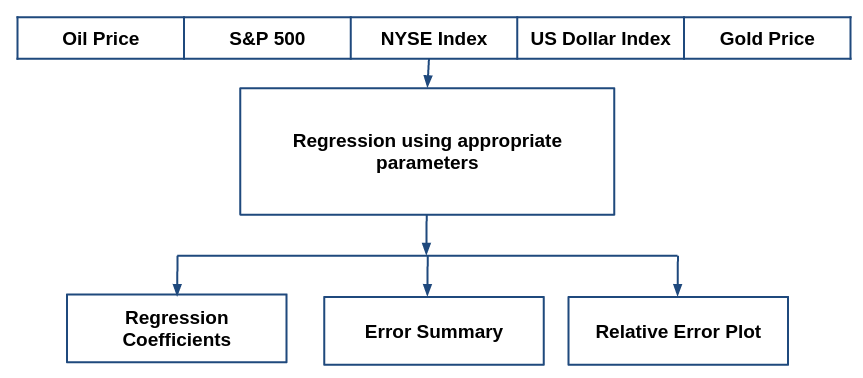
\includegraphics[width=\textwidth]{DevelopmentFlowchart.png}
\caption{The model development process for the oil price prediction with economic factors involved}
\label{fig:DevelopmentFlowchart.png}
\end{figure}

\noindent We synthesize the economic factors for predicing the oil price into a data frame, then we write a function to generate a multiple linear regression model with auto regressive feature [CHECK: is "multiple linear regression model with auto regressive feature" a good alternative wording or shall we continue use "auto regressive model taking economic factors", omitting "linear regression"?]. Then we write a function to run linear regression using appropriate parameters. After executing the function, we obtain the regression coefficients. Based on that, we can continue derive error summaries and make relative error plots. \\

\begin{figure}
\centering
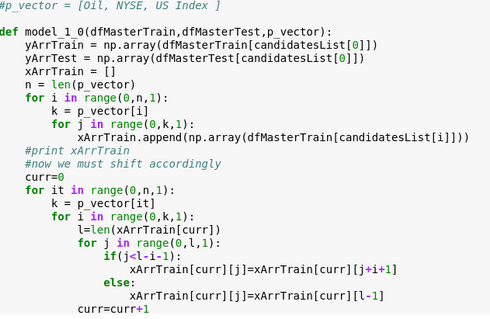
\includegraphics[width=\textwidth]{ModelFunction.png}
\caption{The piece of code of generating a model function}
\label{fig:ModelFunction.png}
\end{figure}

\begin{figure}
\centering
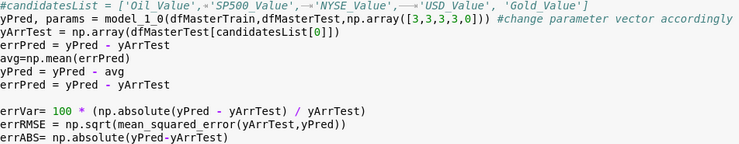
\includegraphics[width=\textwidth]{ErrorCalculation.png}
\caption{The piece of code that calls the model generating function and calculates the errors}
\label{fig:ErrorCalculation.png}
\end{figure}

\begin{figure}
\centering
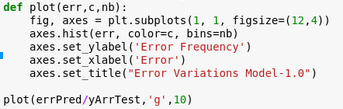
\includegraphics[width=\textwidth]{ErrorPlot.png}
\caption{The piece of code that plots the error distributions}
\label{fig:ErrorPlot.png}
\end{figure}

\textbf{Evaluating the Model:} We train our regression model on 0.6 percent of the time series. We test it on 0.4 percent of the time series. To make sure we are not overfitting our models, we tried cross-validation across the time series (using a k-sized window and sliding it forward). 

\textbf{Error metrics:} We use the mean relative error(percentage error), mean absolute error and RMSE for evaluating the performance of our model. 

\section{Current Model and Baseline}

\subsection{Models using Daily Data}

\noindent\textbf{OIL} \\

% Current Autoregressive Models - Oil%
\noindent\textbf{Current Autoregressive Models} \\
Oil price of last 1 day\\
Mean Relative Error: 0.0310388469621\% \\
Mean Absolute Error:  1.3082794476 \\
RMSE:  1.85081438497 \\
\begin{figure}
\centering
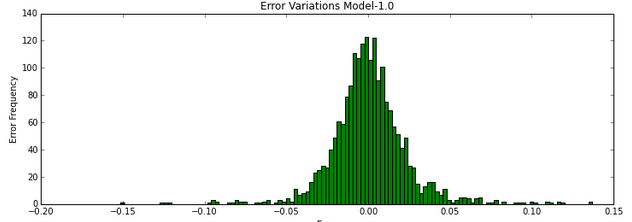
\includegraphics[width=\textwidth]{OilLast1_Daily.png}
\caption{Relative Error Frequency Distribution of Oil price of last 1 day}
\label{fig:OilLast1_Daily.png}
\end{figure}

\noindent Oil price of last 3 days \\
Mean Relative Error: 0.0321107226555\% \\
Mean Absolute Error:  1.3099150004 \\
RMSE:  1.84853705645 \\
\begin{figure}
\centering
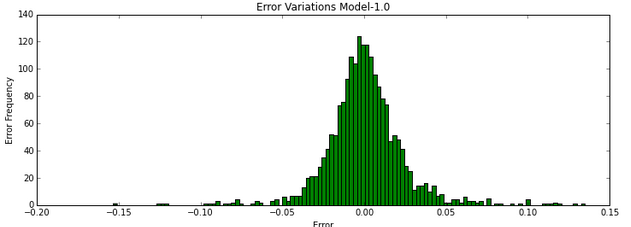
\includegraphics[width=\textwidth]{OilLast3_Daily.png}
\caption{Relative Error Frequency Distribution of Oil price of last 3 days}
\label{fig:OilLast3_Daily.png}
\end{figure}

% Current Multiple Linear Regression Models - Oil%
\noindent\textbf{Current Multiple Linear Regression Models} \\
Oil Price and S\&P 500 Index of past 3 days \\
Mean Relative Error: 0.0311796205698\% \\
Mean Absolute Error: 1.30974996572 \\
RMSE: 1.8455013060818297 \\
\begin{figure}
\centering
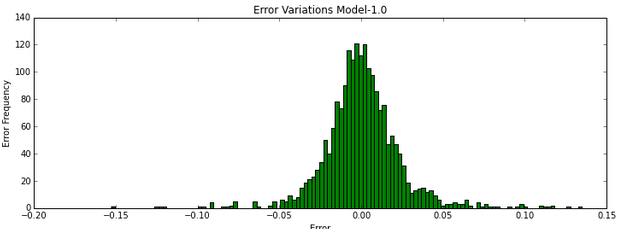
\includegraphics[width=\textwidth]{OilSP500_Daily.png}
\caption{Relative Error Frequency Distribution of Oil Price and S\&P 500 Index of past 3 days}
\label{fig:OilSP500_Daily.png}
\end{figure}

Oil Price and NYSE Index of past 3 days \\
Mean Relative Error: 0.0340500920729\% \\
Mean Absolute Error: 1.30953350368 \\
RMSE: 1.8434889427590628 \\
\begin{figure}
\centering
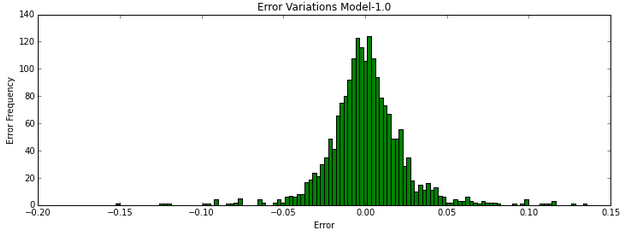
\includegraphics[width=\textwidth]{OILNYSE_Daily.png}
\caption{Relative Error Frequency Distribution of Oil Price and NYSE Index of past 3 days}
\label{fig:OILNYSE_Daily.png}
\end{figure}

Oil Price and USD Index of past 3 days \\
Mean Relative Error: 0.0328232543398\% \\
Mean Absolute Error: 1.30975016152 \\
RMSE: 1.8481711953334485 \\
\begin{figure}
\centering
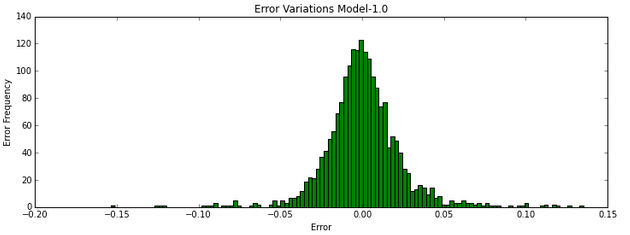
\includegraphics[width=\textwidth]{OILUSD_Daily.png}
\caption{Relative Error Frequency Distribution of Oil Price and USD Index of past 3 days}
\label{fig:OILUSD_Daily.png}
\end{figure}

Oil and Gold price of past 3 days \\ 
Mean Relative Error: 0.0278223283849\% \\
Mean Absolute Error: 1.31597851104 \\
RMSE: 1.85588820013 \\
\begin{figure}
\centering
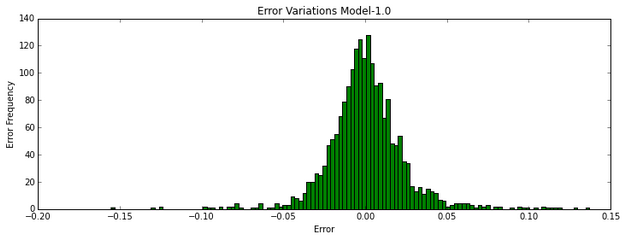
\includegraphics[width=\textwidth]{OILGOLD_Daily.png}
\caption{Relative Error Frequency Distribution of Oil and Gold price of past 3 days}
\label{fig:OILGOLD_Daily.png}
\end{figure}

Oil Price, S\&P 500 and NYSE of past 3 days \\ 
Mean Relative Error: 0.0440463175174\% \\
Mean Absolute Error: 1.31017934091 \\
RMSE: 1.84207587144 \\
\begin{figure}
\centering
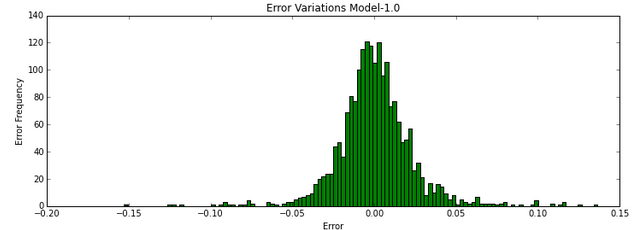
\includegraphics[width=\textwidth]{OILSP500NYSE_Daily.png}
\caption{Relative Error Frequency Distribution of Oil Price, S\&P 500 and NYSE of past 3 days}
\label{fig:OILSP500NYSE_Daily.png}
\end{figure}

Oil Price, S\&P 500 and USD Index of past 3 days \\ 
Mean Relative Error: 0.0330331932997\% \\
Mean Absolute Error: 1.30932708968 \\
RMSE: 1.8443164136 \\
\begin{figure}
\centering
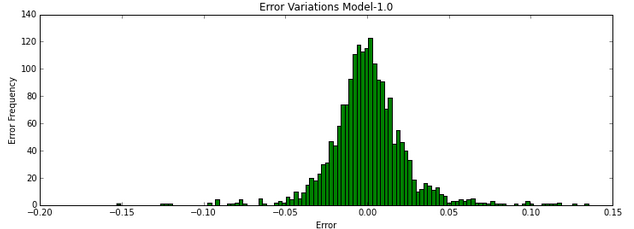
\includegraphics[width=\textwidth]{OILSP500USD_Daily.png}
\caption{Relative Error Frequency Distribution of Oil Price, S\&P 500 and USD Index of past 3 days}
\label{fig:OILSP500USD_Daily.png}
\end{figure}

Oil, S\&P 500 and Gold Price of past 3 days \\ 
Mean Relative Error: 0.00948629213974\% \\
Mean Absolute Error: 1.3226484171 \\
RMSE: 1.86160962907 \\
\begin{figure}
\centering
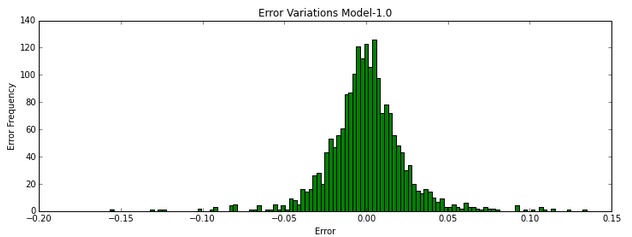
\includegraphics[width=\textwidth]{OILSP500GOLD_Daily.png}
\caption{Relative Error Frequency Distribution of Oil, S\&P 500 and Gold Price of past 3 days}
\label{fig:OILSP500GOLD_Daily.png}
\end{figure}

Oil Price, NYSE and USD Index of past 3 days \\ 
Mean Relative Error: 0.039410146038\% \\
Mean Absolute Error: 1.30918642326 \\
RMSE: 1.84173727654 \\
\begin{figure}
\centering
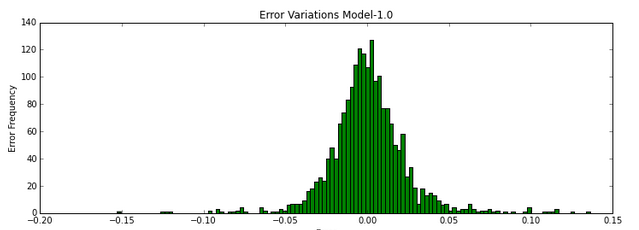
\includegraphics[width=\textwidth]{OILNYSEUSD_Daily.png}
\caption{Relative Error Frequency Distribution of Oil Price, NYSE and USD Index of past 3 days}
\label{fig:OILNYSEUSD_Daily.png}
\end{figure}

Oil Price, S\&P 500, NYSE and USD Index of past 3 days \\ 
Mean Relative Error: 0.0468360442976\% \\
Mean Absolute Error: 1.31001603657 \\
RMSE: 1.84083676985 \\
\begin{figure}
\centering
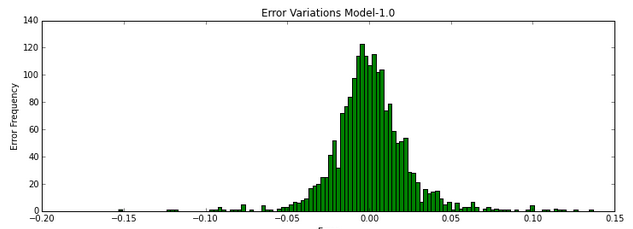
\includegraphics[width=\textwidth]{OILSP500NYSEUSD_Daily.png}
\caption{Relative Error Frequency Distribution of Oil Price, S\&P 500, NYSE and USD Index of past 3 days}
\label{fig:OILSP500NYSEUSD_Daily.png}
\end{figure}

Oil Price, S\&P 500, NYSE, USD Index and Gold Price of past 3 days \\ 
Mean Relative Error: 0.0469027209345\% \\
Mean Absolute Error: 1.31551767844 \\
RMSE: 1.84760329686 \\
\begin{figure}
\centering
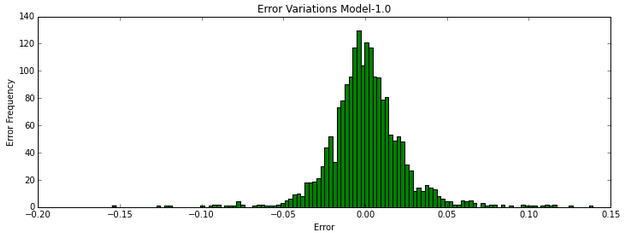
\includegraphics[width=\textwidth]{OILSP500NYSEUSDGOLD_Daily.png}
\caption{Relative Error Frequency Distribution of Oil Price, S\&P 500, NYSE, USD Index and Gold Price of past 3 days}
\label{fig:OILSP500NYSEUSDGOLD_Daily.png}
\end{figure}

\noindent\textbf{Performance against Baseline Models} \\
Current Autoregressive Models against Baseline \\
\begin{figure}
\centering
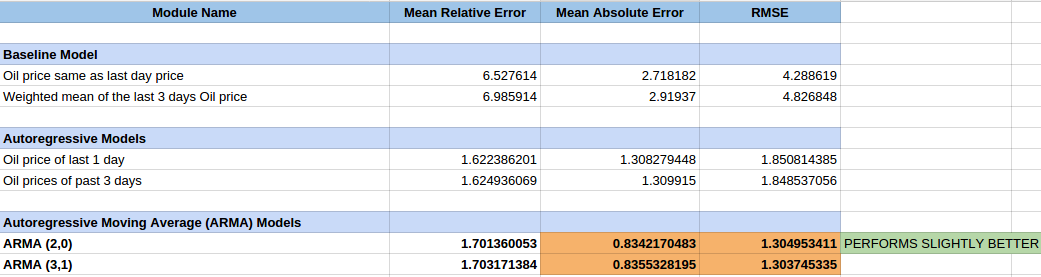
\includegraphics[width=\textwidth]{OILAutoAgainstBase_Daily.png}
\caption{Current Autoregressive Models against base}
\label{fig:OILAutoAgainstBase_Daily.png}
\end{figure}

Current Multiple Linear Regression Models against Baseline \\
\begin{figure}
\centering
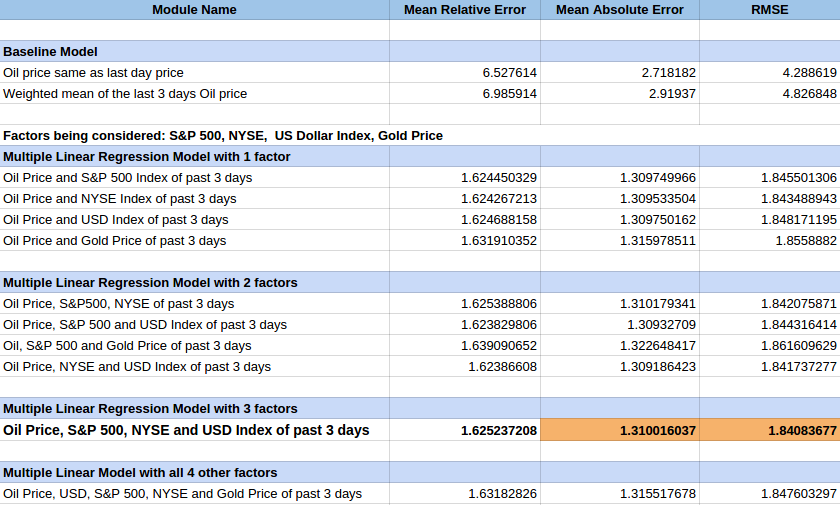
\includegraphics[width=\textwidth]{OILMLRAgainstBase_Daily.png}
\caption{Current Autoregressive Models against base}
\label{fig:OILMLRAgainstBase_Daily.png}
\end{figure}


\noindent\textbf{Comparison Summary} \\
Autoregressive Models "ARMA(2,0)" and "ARMA(3,1)" have lower errors than the baseline models. ARMA(2,0) has slightly lower Mean Relative Error and Mean Absolute Error than ARMA(3,1), but a slightly higher RMSE than ARMA(3,1). \\
Multiple Linear Regression Model "Oil Price, S\&P 500, NYSE and USD Index of past 3 days" has the lowest RMSE. 
It has lower errors than the baseline models. \\

\noindent\textbf{GOLD}
% Current Autoregressive Models - Gold%
\noindent\textbf{Current Autoregressive Models}
Gold price of last 1 day\\
Mean Relative Error: 0.909893675973\% \\
Mean Absolute Error:  10.6253169107 \\
RMSE:  15.6143532961 \\
\begin{figure}
\centering
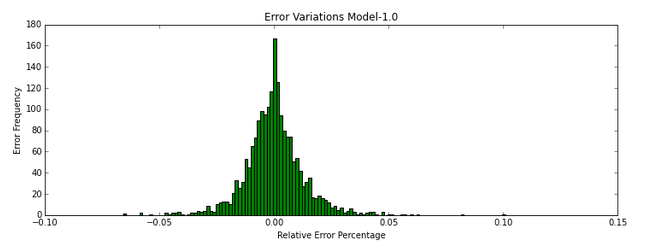
\includegraphics[width=\textwidth]{GoldLast1_Daily.png}
\caption{Relative Error Frequency Distribution of Gold price of last 1 day}
\label{fig:GoldLast1_Daily.png}
\end{figure}

\noindent Gold price of last 3 days \\
Mean Relative Error: 0.911377728085\% \\
Mean Absolute Error:  10.6356749372 \\
RMSE: 15.6120963842 \\
\begin{figure}
\centering
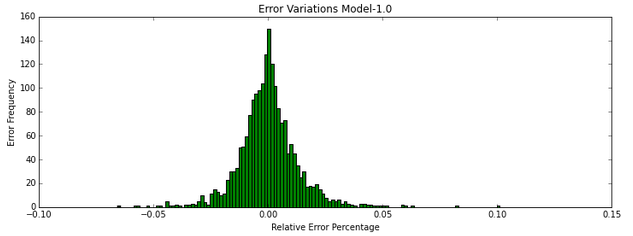
\includegraphics[width=\textwidth]{GoldLast3_Daily.png}
\caption{Relative Error Frequency Distribution of Gold price of last 3 days}
\label{fig:GoldLast3_Daily.png}
\end{figure}

% Current Multiple Linear Regression Models - Gold%
\noindent\textbf{Current Multiple Linear Regression Models}
\noindent Gold Price and S\&P 500 Index of past 3 days \\
Mean Relative Error: 0.910989470538\% \\
Mean Absolute Error:  10.6341118943 \\
RMSE: 15.6150999361 \\
\begin{figure}
\centering
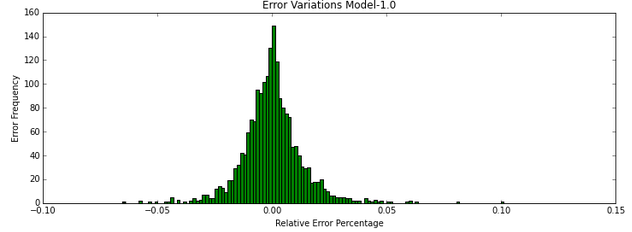
\includegraphics[width=\textwidth]{GoldSP500_Daily.png}
\caption{Relative Error Frequency Distribution of Gold Price and S\&P 500 Index of past 3 days }
\label{fig:GoldSP500_Daily.png}
\end{figure}

\noindent Gold Price and NYSE Index of past 3 days \\
Mean Relative Error: 0.908913469643 \% \\
Mean Absolute Error:  10.6148888844 \\
RMSE: 15.5928578053 \\
\begin{figure}
\centering
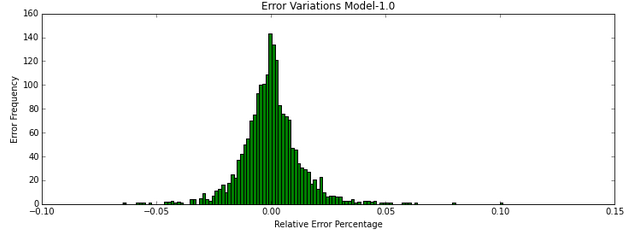
\includegraphics[width=\textwidth]{GoldNYSE_Daily.png}
\caption{Relative Error Frequency Distribution of Gold Price and NYSE Index of past 3 days}
\label{fig:GoldNYSE_Daily.png}
\end{figure}

\noindent Gold Price and USD Index of past 3 days \\
Mean Relative Error: 0.910740053257\% \\
Mean Absolute Error:  10.62421809 \\
RMSE: 15.6011151411 \\
\begin{figure}
\centering
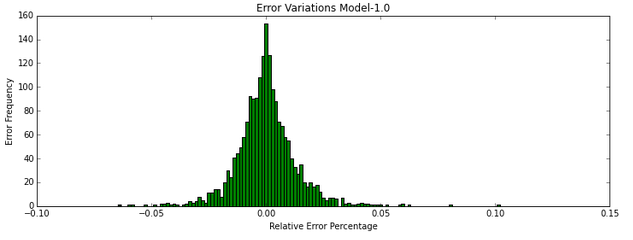
\includegraphics[width=\textwidth]{GoldUSD_Daily.png}
\caption{Relative Error Frequency Distribution of Gold Price and USD Index of past 3 days}
\label{fig:GoldUSD_Daily.png}
\end{figure}

\noindent Gold Price and Euro/USD Exchange Rate of past 3 days \\
Mean Relative Error: 0.913922103832\% \\
Mean Absolute Error:  10.6570840116 \\
RMSE: 15.6285864477 \\
\begin{figure}
\centering
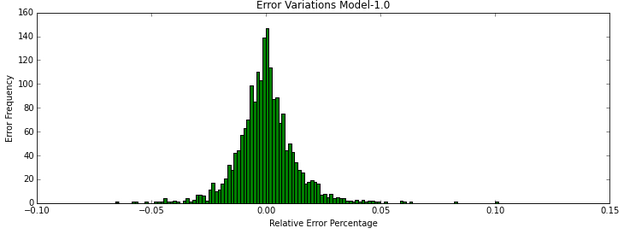
\includegraphics[width=\textwidth]{GoldEuro_Daily.png}
\caption{Relative Error Frequency Distribution of Gold Price and Euro/USD Exchange Rate of past 3 days}
\label{fig:GoldEuro_Daily.png}
\end{figure}

\noindent Gold Price and CSI of past 3 days \\
Mean Relative Error: 0.911209607511\% \\
Mean Absolute Error:  10.6331605485 \\
RMSE: 15.6116052727 \\
\begin{figure}
\centering
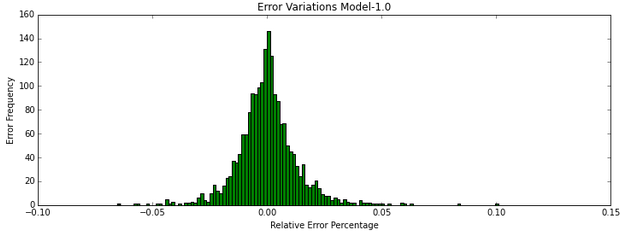
\includegraphics[width=\textwidth]{GoldCSI_Daily.png}
\caption{Relative Error Frequency Distribution of Gold Price and CSI of past 3 days}
\label{fig:GoldCSI_Daily.png}
\end{figure}

\noindent Gold Price and Oil Price of past 3 days \\
Mean Relative Error: 0.906189820768 \% \\
Mean Absolute Error: 10.5847085212 \\
RMSE: 15.5115814636 \\
\begin{figure}
\centering
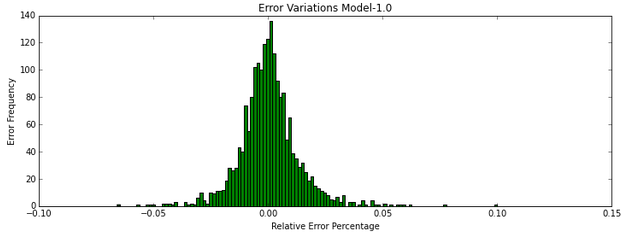
\includegraphics[width=\textwidth]{GoldOil_Daily.png}
\caption{Relative Error Frequency Distribution of Gold Price and Oil Price of past 3 days}
\label{fig:GoldOil_Daily.png}
\end{figure}

Note: After generating the correlation coefficient heat map [Fig 4.], we only concerning the combination of Gold Price, USD, EURO/USD, CSI, Oil Price for predicting gold price. \\

\noindent Gold Price, USD and EURO/USD of past 3 days \\
Mean Relative Error: 0.909034610537\% \\
Mean Absolute Error:  10.6077232979 \\
RMSE: 15.5861191185 \\
\begin{figure}
\centering
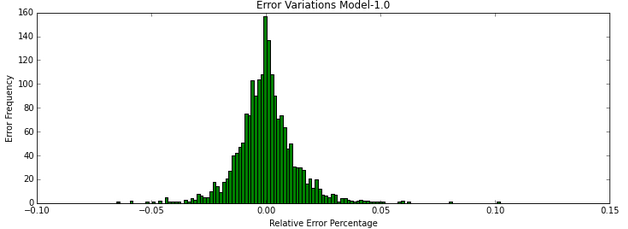
\includegraphics[width=\textwidth]{GoldUSDEuro_Daily.png}
\caption{Relative Error Frequency Distribution of Gold Price, USD and EURO/USD of past 3 days}
\label{fig:GoldUSDEuro_Daily.png}
\end{figure}

\noindent Gold Price, USD and CSI of past 3 days \\
Mean Relative Error: 0.910204441426\% \\
Mean Absolute Error: 10.618696403 \\
RMSE: 15.5998214307 \\
\begin{figure}
\centering
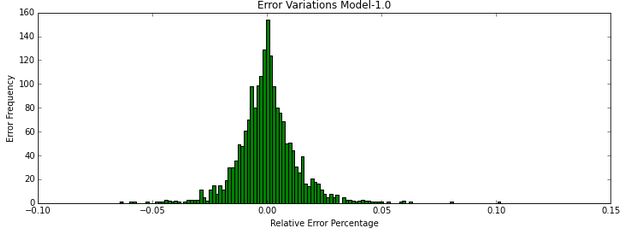
\includegraphics[width=\textwidth]{GoldUSDCSI_Daily.png}
\caption{Relative Error Frequency Distribution of Gold Price, USD and CSI of past 3 days}
\label{fig:GoldUSDCSI_Daily.png}
\end{figure}

\noindent Gold Price, USD and Oil Price of past 3 days \\
Mean Relative Error: 0.907577054439\% \\
Mean Absolute Error: 10.5947059823 \\
RMSE: 15.508598881 \\
\begin{figure}
\centering
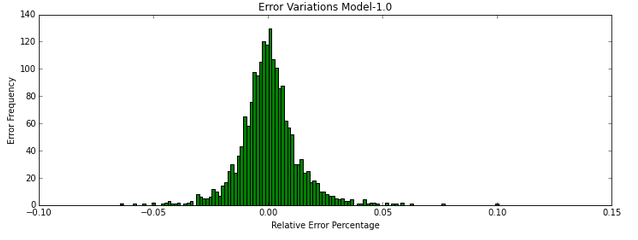
\includegraphics[width=\textwidth]{GoldUSDOil_Daily.png}
\caption{Relative Error Frequency Distribution of Gold Price, USD and Oil Price of past 3 days}
\label{fig:GoldUSDOil_Daily.png}
\end{figure}

\noindent Gold Price, EURO/USD and CSI of past 3 days \\
Mean Relative Error: 0.913284526674\% \\
Mean Absolute Error: 10.6489809425 \\
RMSE: 15.6247642766 \\
\begin{figure}
\centering
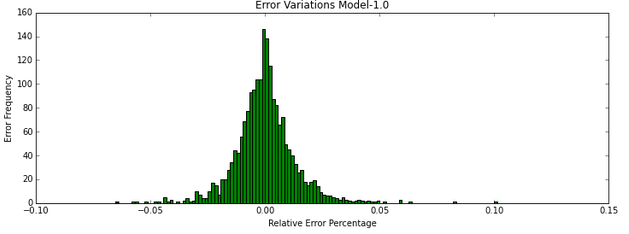
\includegraphics[width=\textwidth]{GoldEuroCSI_Daily.png}
\caption{Relative Error Frequency Distribution of Gold Price, EURO/USD and CSI of past 3 days}
\label{fig:GoldEuroCSI_Daily.png}
\end{figure}

\noindent Gold Price, EURO/USD and Oil Price of past 3 days \\
Mean Relative Error: 0.908706241253\% \\
Mean Absolute Error:  10.6092302631 \\
RMSE: 15.5220108937 \\
\begin{figure}
\centering
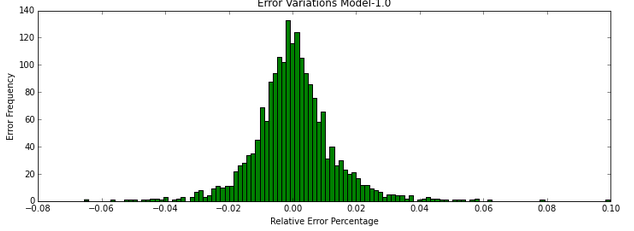
\includegraphics[width=\textwidth]{GoldEuroOil_Daily.png}
\caption{Relative Error Frequency Distribution of Gold Price, EURO/USD and Oil Price of past 3 days}
\label{fig:GoldEuroOil_Daily.png}
\end{figure}

\noindent Gold Price, CSI and Oil Price of past 3 days \\
Mean Relative Error: 0.906784413338\% \\
Mean Absolute Error: 10.5903571944 \\
RMSE: 15.516795603 \\
\begin{figure}
\centering
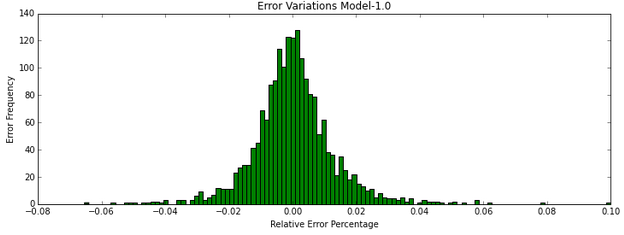
\includegraphics[width=\textwidth]{GoldCSIOil_Daily.png}
\caption{Relative Error Frequency Distribution of Gold Price, CSI and Oil Price of past 3 days}
\label{fig:GoldCSIOil_Daily.png}
\end{figure}

\noindent Gold Price, USD, EURO/USD and CSI of past 3 days \\
Mean Relative Error: 0.908442364248\% \\
Mean Absolute Error: 10.6013470188 \\
RMSE: 15.580032763 \\
\begin{figure}
\centering
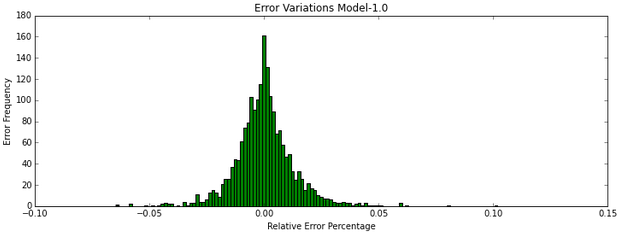
\includegraphics[width=\textwidth]{GoldUSDEuroCSI_Daily.png}
\caption{Relative Error Frequency Distribution of Gold Price, USD, EURO/USD and CSI of past 3 days}
\label{fig:GoldUSDEuroCSI_Daily.png}
\end{figure}

\noindent Gold Price, USD, EURO/USD and Oil Price of past 3 days \\
Mean Relative Error: 0.907727253341\% \\
Mean Absolute Error: 10.5956228326\\
RMSE: 15.506047026 \\
\begin{figure}
\centering
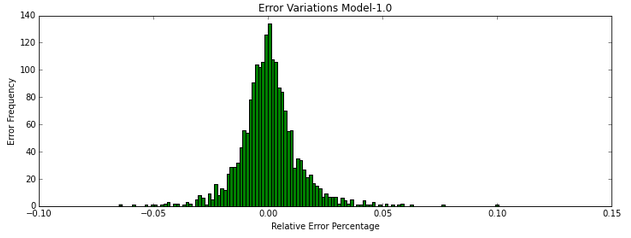
\includegraphics[width=\textwidth]{GoldUSDEuroOil_Daily.png}
\caption{Relative Error Frequency Distribution of Gold Price, USD, EURO/USD and Oil Price of past 3 days}
\label{fig:GoldUSDEuroOil_Daily.png}
\end{figure}

\noindent Gold Price, USD, CSI and Oil Price of past 3 days \\
Mean Relative Error: 0.908974041264\% \\
Mean Absolute Error:  10.6083836761 \\
RMSE: 15.5197835526 \\
\begin{figure}
\centering
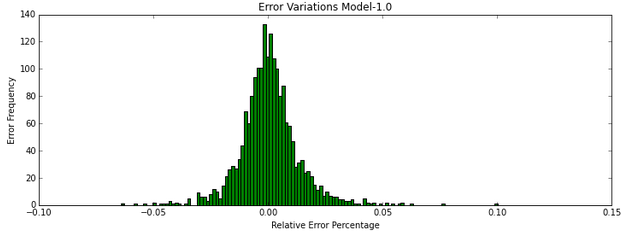
\includegraphics[width=\textwidth]{GoldUSDCSIOil_Daily.png}
\caption{Relative Error Frequency Distribution of Gold Price, USD, CSI and Oil Price of past 3 days}
\label{fig:GoldUSDCSIOil_Daily.png}
\end{figure}

\noindent Gold Price, EURO/USD, CSI and Oil Price of past 3 days \\
Mean Relative Error: 0.909469026042 \% \\
Mean Absolute Error: 10.6164466869 \\
RMSE: 15.5296531045 \\
\begin{figure}
\centering
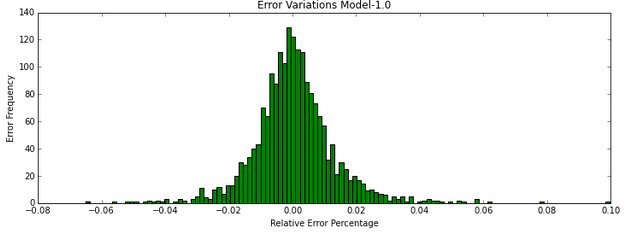
\includegraphics[width=\textwidth]{GoldEuroCSIOil_Daily.png}
\caption{Relative Error Frequency Distribution of Gold price of last 3 days}
\label{fig:GoldEuroCSIOil_Daily.png}
\end{figure}

\noindent Gold Price, USD, EURO/USD, CSI and Oil Price of past 3 days \\
Mean Relative Error: 0.907849241727 \% \\
Mean Absolute Error: 10.5960848588 \\
RMSE: 15.5083690942 \\
\begin{figure}
\centering
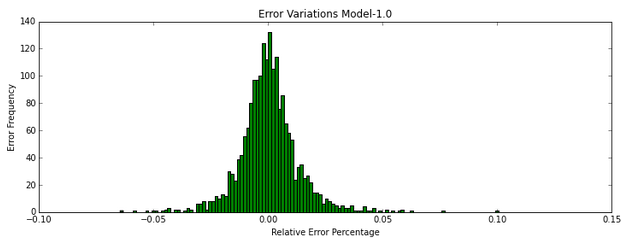
\includegraphics[width=\textwidth]{GoldUSDEuroCSIOil_Daily.png}
\caption{Relative Error Frequency Distribution of Gold Price, USD, EURO/USD, CSI and Oil Price of past 3 days}
\label{fig:GoldUSDEuroCSIOil_Daily.png}
\end{figure}

\noindent\textbf{Performance against Baseline Models}
Current Autoregressive Models against Baseline \\
\begin{figure}
\centering
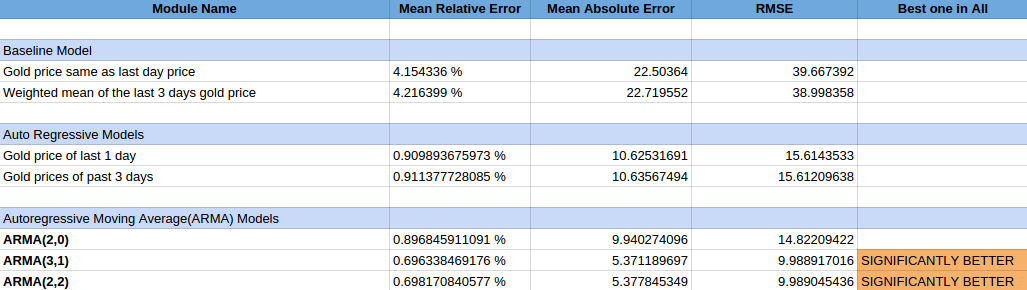
\includegraphics[width=\textwidth]{GoldAutoAgainstBase_Daily.png}
\caption{Current Autoregressive Models against base}
\label{fig:GoldAutoAgainstBase_Daily.png}
\end{figure}

Current Multiple Linear Regression Models against Baseline \\
\begin{figure}
\centering
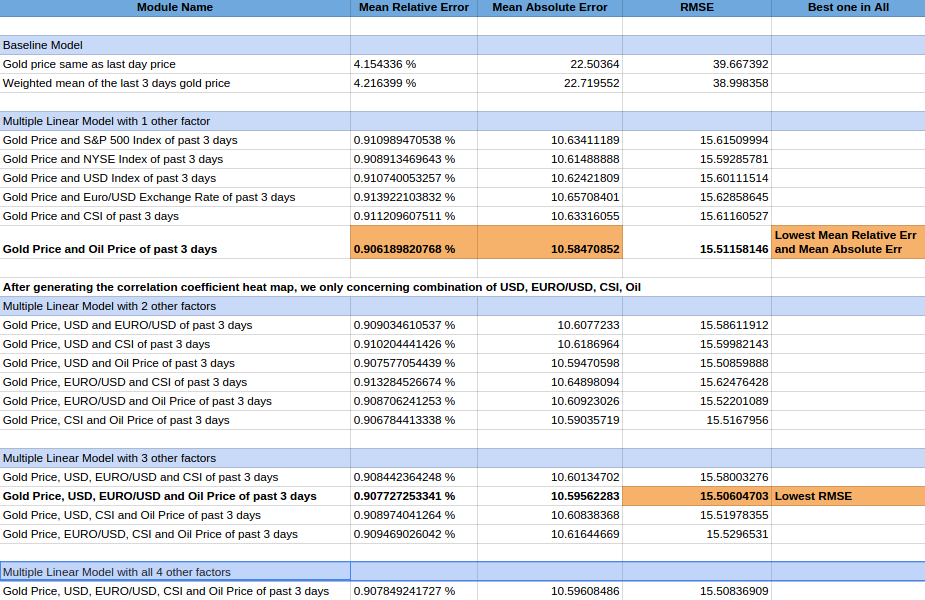
\includegraphics[width=\textwidth]{GoldMLRAgainstBase_Daily.png}
\caption{Current Autoregressive Models against base}
\label{fig:GoldMLRAgainstBase_Daily.png}
\end{figure}

\noindent\textbf{Comparison Summary} \\
Autoregressive Models "ARMA(3,1)" and "ARMA(2,2)" have significantly lower errors than the baseline models. ARMA(3,1) has slightly lower errors 
than ARMA(2,2). \\
Multiple Linear Regression Model "Gold Price and Oil Price of past 3 days" has the lowest mean relative error and the lowest mean absolute error; 
 "Gold Price, USD, EURO/USD and Oil Price of past 3 days" has the lowest RMSE.
Both have significant lower errors than the baseline models. \\

\subsection{Models using Monthly Data}

\noindent\textbf{OIL}

\noindent\textbf{Current Autoregressive Models}

\noindent\textbf{Current Multiple Linear Regression Models}

\noindent\textbf{Performance against Baseline Models}

\noindent\textbf{Comparison Summary}


\noindent\textbf{GOLD}

\noindent\textbf{Current Autoregressive Models}

\noindent\textbf{Current Multiple Linear Regression Models}

\noindent\textbf{Performance against Baseline Models}

\noindent\textbf{Comparison Summary}


\subsection{Overall Summary}


\section{Current Prediction and Next Steps}

Predicted price of WTI Crude Oil on Dec 1 as of Nov 1 is \\
\textbf{93.7 USD per Barrel} \\

\noindent Predicted price of Gold on Dec 1 as of Nov 1 \\
\textbf{1240.6 USD per ounce} \\

\noindent We will further investigate how we may include futures price as one of the economic factors to help predict oil and gold price. \\

\noindent [ADD "Present what you will do next to get a complete predictive model.  Discuss any difficulties you will have to overcome in building a good model"]

\subsubsection*{Acknowledgments.} Here acknowledge any other people who helped with this project.

\section{Bibliography}\label{references}

The correct BibTeX entries for the Lecture Notes in Computer Science
volumes can be found at the following Website shortly after the
publication of the book:
\url{http://www.informatik.uni-trier.de/~ley/db/journals/lncs.html}

For citations in the text please use
square brackets and consecutive numbers: \cite{jour}, \cite{lncschap},
\cite{proceeding1} -- provided automatically
by \LaTeX 's \verb|\cite| \dots\verb|\bibitem| mechanism.

Please base your references on the
examples below. 
The following section shows a sample reference list with entries for
journal articles \cite{jour}, an LNCS chapter \cite{lncschap}, a book
\cite{book}, proceedings without editors \cite{proceeding1} and
\cite{proceeding2}, as well as a URL \cite{url}.
Please note that proceedings published in LNCS are not cited with their
full titles, but with their acronyms!

\begin{thebibliography}{4}

\bibitem{jour} Smith, T.F., Waterman, M.S.: Identification of Common Molecular
Subsequences. J. Mol. Biol. 147, 195--197 (1981)

\bibitem{lncschap} May, P., Ehrlich, H.C., Steinke, T.: ZIB Structure Prediction Pipeline:
Composing a Complex Biological Workflow through Web Services. In: Nagel,
W.E., Walter, W.V., Lehner, W. (eds.) Euro-Par 2006. LNCS, vol. 4128,
pp. 1148--1158. Springer, Heidelberg (2006)

\bibitem{book} Foster, I., Kesselman, C.: The Grid: Blueprint for a New Computing
Infrastructure. Morgan Kaufmann, San Francisco (1999)

\bibitem{proceeding1} Czajkowski, K., Fitzgerald, S., Foster, I., Kesselman, C.: Grid
Information Services for Distributed Resource Sharing. In: 10th IEEE
International Symposium on High Performance Distributed Computing, pp.
181--184. IEEE Press, New York (2001)

\bibitem{proceeding2} Foster, I., Kesselman, C., Nick, J., Tuecke, S.: The Physiology of the
Grid: an Open Grid Services Architecture for Distributed Systems
Integration. Technical report, Global Grid Forum (2002)

\bibitem{url} National Center for Biotechnology Information, \url{http://www.ncbi.nlm.nih.gov}

\end{thebibliography}


\end{document}
